\documentclass[letterpaper]{article} % Feel free to change this
\usepackage{epsfig}

\begin{document}

\title{ECE 350: Digital Systems Processor Technical Report}
\author{Mary Stuart Elder} % Change this to your name
\date{October 30, 2018} % Change this to the date you are submitting
\maketitle

\section{Introduction}

By submitting this \LaTeX{} document, I affirm that
\begin{enumerate}
    \item I understand that each \texttt{git} commit I create in this repository is a submission
    \item I affirm that each submission complies with the Duke Community Standard and the guidelines set forth for this assignment
    \item I further acknowledge that any content not included in this commit under the version control system cannot be considered as a part of my submission.
    \item Finally, I understand that a submission is considered submitted when it has been pushed to the server.
\end{enumerate}

\section{Introduction}
The following technical report details the implementation of my processor. The general design is a 5 stage pipeline with bypassing, branch prediction, and an ALU with a carry-select / carry-lookahead adder. I will detail my implementation in the following pages.

\section{Subcomponents}
\subsection{Regfile}
\subsubsection{Write Port}
After the initial variable declarations, my regfile.v code begins by creating the write port. This is done by calling both the decode5to32 module and the decodeANDwe module. The first module is a general 5 to 32 decoder made of NOT and AND gates. The second module takes each bit of the decoder's output and ANDs it with the write enable from regfile to create write enables for each register. The exception is the 0th bit, which is ANDed with a 0 to ensure register 0 is not overwritten.
\subsubsection{Read Ports}
Once the write port is established, the read ports are created by using the same decode5to32 module as before. The resulting readDecodeA and readDecodeB vectors are used in the generate loop. In this loop, they are used as the enable signal to the 32-bit tristate buffer module.
\subsubsection{Generate Loop}
The generate loop instantiates my 32 registers. The register, found in register.v, is made from 32 instantiations of the dffe-ref module provided. The corresponding write enable signal is given to each register by the genvar value. The value in regOut is sent to two 32-bit tristate buffers (as mentioned above). These buffers, found in the tri32.v file, were made from 32 assign statements. This allows a 32-bit input to effectively enter 1 tristate buffer. If the readDecodeA or readDecodeB value corresponds to the given register, it will pass through the tristate buffer and drive the data-readRegA or data-readRegB outputs.
\subsubsection{Clocking Estimation}
Based on testbench tests of this specific component, my register file can be clocked at 19.3ns. I modified the clock in the testbench multiple times. My code began throwing errors when the clock variable fell below 9.65, so I estimate my clock speed to be 19.3ns.

\subsection{ALU}
\subsubsection{alu.v}
The general structure of my alu is the connection of a CLA/CS adder, 32 bit AND, 32 bit OR, and two barrel shifters to tristate buffers. These tristate buffers, controlled by a decoded ALU opcode, send data to the data-result bus. I also have tristate buffers for the control bits: isLessThan, isNotEqual, and overflow. I calculated isNotEqual by instantiating the notEqual module in the ALU module to enhance timing. If the opcode dictates an add or subtract, I send the overflow output of the adder to the overflow control bit. If the opcode dictates a subtract specifically, I also send the isnotequal and islessthan outputs of the adder to the control bits. The exception to this is when data-operandA and data-operandB both equal zero and the opcode dictates a subtraction. This case leads to long calculations of carries just to send all 0s to the outputs. Therefore, I hard coded a catch for these inputs and sent all zero results in this case.
\subsubsection{translateOpcode.v}
This module takes the ALU-opcode and, using the assignments given in the lab report, creates a 6 bit "modEnable" variable. Each ALU command has a given enable bit from this variable at a given index as seen in the comments of the code.

\subsubsection{cla-cs-adder.v}
I implemented the carry lookahead adder with 7 x 8-bit CLA blocks, explained below, to create a hierarchical carry lookahead adder with carry-select elements. While the overall carry bits are being calculated, the carry-select portion generates options for the sum. The carry bits then act as control bits for these options. The adder module also contains logic for creating the overflow and isLessThan control bits in the alu module. These results are sent to the alu file.

\subsubsection{cla-8block.v}
Each CLA block creates the carry bits in parallel using the outputs of the 32-bit AND and ORs. These carries are used to create the sum output bits in a generate loop.

\subsubsection{notEqual.v}
My notEqual module takes the two data inputs, performs a bitwise XOR, ORs the outputs of the XORs, and NOTs this output. This will be 1 if any bits of the inputs do not match.

\subsubsection{and/or/not/tri32.v}
The tri32 module is the same as in the regfile, so it contains 32 tristate statements to send the input if the control is 1 and z otherwise. The and, or, and not32 modules use generate loops to instantiate bitwise AND, OR, and NOTs.

\subsubsection{tri8.v}
This is essentially a mux for 2 8bit inputs.

\subsubsection{barrelShiftL.v and associated shiftLby files}
I used these files to implement my 32 bit SLL barrel shifter. The submodules for the left barrel shifter "copy" the data from the lower end of the input data into the upper end of the output data. Then, the final lower bits of the output data (for shiftLby16, lower 16 bits, for shiftLby8, lower 8 bits) are filled with 0s. This is implemented via two generate loops with AND statements using the input output and sending it to the output data. The final output is generated by instantiating each shifter submodule, connecting shifted and unshifted data options to "muxes" (tristate buffers controlled by shiftamt), and stringing these shifter submodules together as follows: 16 - 8 - 4 - 2 - 1.

\subsubsection{barrelShiftR.v and associated shiftRby files}
I used these files to implement my 32 bit SRA barrel shifter. The submodules for the right barrel shifter "copy" the data from the upper end of the input data into the lower end of the output data. Then, the most significant bit (dataIn[31]) is copied into the final upper bits of the output data (for shiftRby16, upper 16 bits, for shiftRby8, upper 8 bits). This is implemented via two generate loops with AND statements using the input output and sending it to the output data. The overall structure of the barrelshiftR follows that of barrelShiftL.

\subsubsection{Errors fixed from pc2}
At the time of submission for pc2, my ALU had an error in the carry logic. A single variable that was needed for the logic was not included originally. I amended this for the version of the ALU in my processor.

\subsubsection{Timing}
I estimate my ALU to clock at 18.7ns. This is based on running the testbench in small increments until I received error messages. I pass all of the testbench tests.

\subsection{Mult/Div}
The final design of my processor treated mul and div operations as add and sub operations, respectively. This design choice stemmed from the functionality of my multdiv module as submitted in the third project checkpoint. Although the module functioned well and passed all local tests, it triggered hold time violations when run on the TA testers. I approached several TAs for guidance regarding these errors and was advised to prioritize the rest of the functioning processor over fixing the hold time violation. Since no TAs understood the source of my errors, I decided to code my control module to catch mul/div operations and create controls as though they were add/sub.
\subsection{Memory Elements}
I generated my memory elements using the RAM: 1-port megafunction. The memory elements have data in/output buses 32 bits wide, 12 bit address inputs, and write enables (although imem does not utilize the write enable or data in). Both memory elements also utilize a single clock. The output ports of the imem and dmem are not registered. I clocked these elements to the positive edge to get correct outputs locally.

\section{Full processor}
\subsection{Design implementation: F}
The fetch portion of my design contains a few main components.
\subsubsection{PC Latch}
The PC register/latch (pcReg) keeps track of the current program count and is a simple 32 bit register. The output of this register feeds into a branch predictor module, an ALU, and the imem module in the skeleton file.
\subsubsection{ALU}
The ALU component adds 1 to the program count, since memory is word addressed. 
\subsubsection{Branch Predictor}
For a read, the branch predictor takes in the lower 12 bits (address portion) of the output of the PC latch and uses the bottom 5 bits to index 32 registers. This format is similar to reading in the regfile, but using 12 bit registers rather than 32. Once the register corresponding to the lower 5 bits of the address is found, its output is sent out of the branch predictor, as is the output of its corresponding "taken" D-flip-flop. Writing to the branch predictor will be explained in the execute phase.
\subsubsection{Imem}
The lower 12 bits of the current PC latch output are set to address-imem in order to extract the correct data from the imem module. This imem output is fed into a mux (along with a nop) controlled by flush logic determined later.
\subsubsection{FD Latch}
My FD latch contains registers storing the following information: the output of the branch predictor/PC + 1 mux; the PC for the corresponding instruction; PC + 1; and the current instruction. The first three pieces of information all come into play for the branch predictor logic later on.

\subsection{Design implementation: D}
The decode phase of my processor contains the following key components: an ALU; interactions with the regfile (from the skeleton); a stall module; a control module; and a DX latch.
\subsubsection{ALU}
This ALU exists to take the PC + 1 output from the FD latch and add the sign extended immediate value (N) to it (PC + 1 + N). I implemented this ALU in the decode phase to limit the processor to 1 ALU per phase. Additionally, branching logic dependent on PC + 1 + N in the X phase is faster this way.
\subsubsection{Regfile interactions: Muxes}
The regfile interactions in the decode phase largely deal with \$rs and \$rt. The decisions for \$rd and the data written to it are made in the W phase. \$rs and \$rt are decided based on 
\subsubsection{Stall Module}
This module will be explained in the "Hazard Handling" section below.
\subsubsection{Control Module}
My control module uses the instruction (IR) output of the FD latch to create the majority of the mux controls for the processor. These controls are either used in the decode phase immediately or are propagated through the pipeline through the DX / XM / MW latches. Figure \ref{fig:1} in the Appendix shows a table of all of the controls generated (apart from the instruction type) for each instruction input. The instruction type output is used mostly for exception detection in the writeback phase. This way, simply checking one bit can determine what value to write back in the case of an exception, since each instruction has a unique bit.
\subsubsection{DX Latch}
The DX latch is the largest of the latches. This is due to the many D-flip-flops storing control bits from the control module. The DX latch also stores the addresses needed for the branch predictor (TG - taken guess, PC, PC + 1) as well as the PC + 1 + Immediate value needed for branch logic.

\subsection{Design implementation: X}
\subsubsection{ALU}
This ALU takes the dataInA wire and the dataInB wire and performs the operation determined by the ALUop output of the DX latch.
\subsubsection{Bypass Module}
The bypass module will be explained further in the "Bypassing Logic" portion below, but the outputs of this bypass module determine the values sent from the dataInA mux and dataInB mux.
\subsubsection{Branch/Jump Muxes}
These muxes choose between the corresponding target of the branch / jump in question (based on the instruction format). The muxes are controlled by the control bits and, for branching, the not equal and/or is less than outputs of the ALU. These muxes output to "myMux2" all the way back in the fetch phase. If the predictor was right, this mux will continue fetching in its usual flow. The next section describes what happens on a misprediction.

\subsubsection{Writing to Branch Predictor}
If the predictor was wrong, the flush logic is updated to send nops to F and D (flush) and the next PC is determined by the correct output of the branch / jump logic. The branch predictor takes in the correct branch address, the original PC resulting in a branch, the PC + 1 value from this same PC, and a bit indicating whether the guess was right or not. The original PC is used to index the register and D-flip-flop corresponding to the correct branch address. This PC is decoded and ANDed with the indicator bit to create a 32 bit write enable for the registers/D-flip-flops in the branch predictor. The correct address is compared to the PC + 1 input. If these are equal, the guessed direction must have been "taken" when it should have been "not taken." Otherwise, the branch address was wrong. Therefore, the correct D-flip-flop is written to with the not of this equality check. The correct register is written to with the correct branch address. 

\subsubsection{XM Latch}
The XM latch holds many control bits for the M and W phases of the pipeline, as well as the PC + 1 value for the W phase of the pipeline to use. The data outputs from the X phase are also held here.

\subsection{Design implementation: M}
The M phase of the pipeline is short and consists of wire assignments for DMEM, a mux, and the MW latch.
\subsubsection{Interactions with DMEM}
address-dmem is assigned to the lower 12 bits of the O output of the XM latch.
\subsubsection{Memory Mux}
This mux chooses between the B output of the XM latch and the bypassed writeback value. The mux is controlled by the DMwe output from the XM latch.
\subsubsection{MW Latch}
The MW latch holds the control bits and PC + 1 value needed for the W phase of the pipeline, as well as the data outputs from the M phase.

\subsection{Design implementation: W}
\subsubsection{Writeback Muxes}
Many controls compete for the writeback value. Initially, the writeback value is determined by muxes between the O and D outputs of the MW latch or PC + 1 (for jal). After these muxes, the writeback value goes through a series of muxes for exception writebacks. This way, the exception has priority. A total of 8 muxes were used for the various exception values and other writeback options.
\subsubsection{\$rd Muxes}
\$rd was determined by two muxes. Overall, the output had the following options: \$rd according to the instruction; \$r31; or \$r30. The controls for these muxes were generated by the control module.
\subsection{Hazard Handling}
\subsubsection{nop}
I created a nop instruction with an opcode of 00000 and an ALU opcode of 01000. My control module took this input to mean no special flags or signals should be asserted. This has the effect of a nop, since nothing is modified. I used this in my flush logic to handle hazards.
\subsubsection{Bypassing / Stalls}
Stalls were implemented with nops in cases when bypassing was insufficient. My stall module generates a control to send a nop if a load operation is followed by something other than a store. This is specific to non-store operations with source registers equal to the destination register from the load. The isStall output of the stall module is fed into the flush logic for sending nops. The nisStall output is fed to the write enable of the FD and DX latches, so the latch is enabled as long as there is no stall. Bypassing prevents the need for many stalls, despite the hazard existing, and will be explained more below. 

\subsection{Minimum Functional Clock Speed}
I estimate 

\subsection{Bypassing logic}
Four muxes were controlled by the bypass logic generated in my bypass module. The muxes for the A / B data in the ALU were controlled by bypass logic. These muxes allow for MX and WX bypassing of data into the alu inputs. The third mux controlled by this logic is for memory. The B input of the data memory has the option of MW bypassing (since this is passing data to data, and not an address). Finally, bypass logic allows a bex operation to occur immediately after a setx operation. The opcodes of the operations were compared to generate the control bits. XM and XW bypassing is possible and was implemented by taking the T portions of the IR outputs of the XM / MW latches and bypassing them to the X phase. This bypassing is disabled if an exception occurs (using the MathExcep control bit from the latches). Instructions following an exception will read the original, unmodified \$rs or \$rt.

\subsection{Efficiency details}
The bypassing implemented in my processor prevents many of the possible stalls due to hazards. However, some causes of inefficiency could be the many casading muxes in my design, multiple ALUs, and the Branch Predictor module/logic. With regards to muxes, the writeback logic is the biggest problem. The output must channel through each of the 8 muxes in order to make it back to the regfile output. Multiple ALUs offers some efficiency benefits, since the resources are dispersed between phases. There is an added hardware cost to this from the extra ALU modules and the added registers needed to store this data. Finally, the branch predictor can cause further inefficiencies in some instruction orders. If multiple branches were included in a code, but each executes exactly once, the branch predictor would never get to learn this behavior and would mispredict every time. Fast branches may be faster in general than this implementation. However, multiple accesses of the same branch will be faster with this method of branching and will cause fewer flushed instructions. 

\section{Instruction Implementation}
\subsection{Include details about how you implemented each instruction}
The control module explanation above begins to explain how I implemented each instruction. I treated each instruction as a signal to trigger specific mux controls / flags scattered through my pipeline. The table detailing these flags can be seen in Figure \ref{fig:1}. The only exceptions to this rule are "mul" and "div". Since I did not include my multdiv, I used my control module to catch these instructions and translate their corresponding control signals (ALUop and Write Enable (WE)) to those of add and sub, respectively.

\section{Process}
\subsection{Why did you choose your implementation?}
I chose to leave out my multdiv module for the reasons explained in the multdiv section above. I chose to implement a branch predictor, rather than fast branching or some other method, in part to make up for not including the multdiv, and in part because the interconnected pipeline made the most sense to me with a branch predictor. I designed my processor file to be as modular as possible because my multdiv was messy and ended up having hold time issues. With modularity, I hoped to avoid that.

\subsection{How did you test your implementation?}
I tested my processor through waveforms from the skeleton file and many variations of imem.mif files. I bubbled up inputs / outputs from the processor file (particularly IR latch outputs) to ensure instructions were properly propagating through the pipeline. I caught many issues through this, particularly lines of code I had thought of but forgot to write initially. An example of one of these waveforms can be found in the Appendix (Figure \ref{fig:2}).

\subsection{Known Errors}
\subsubsection{First Instruction: 0 plus 0}
On start up, the portion of the pipeline dedicated to the instruction is initialized to 0. This non-instruction (32'b0) is interpreted by the processor as add \$0, \$0, \$0. Therefore, the write enable flag is triggered one cycle before the first legitimate instruction makes it through the MW latch. This flaw has no impact on the functioning of the processor (since writing to \$0 does nothing), but it does cause a misleading write enable flag. I found this error in the screenshot provided in the Appendix, Figure \ref{fig:2}. Since the functionality was not affected by this bug, I did not modify the code. However, this bug could be fixed by tying the control generator module to the PC latch output so the control module waits to output actual controls until the true first instruction from the PC begins to propagate. 

\subsection{Challenges - what were the main challenges you faced and how did you
overcome them?}
The hardest part about this project was keeping track of all of the wires and modules running in the processor file. I dealt with this challenge by keeping track of control bits, instructions, and the meaning of various controls in Excel sheets. I also referenced my Logisim processor from ECE 250 to better visualize the flow of the pipeline, since visualizing the pipeline was difficult at times.

\subsection{Main learning points - what did you learn by making this processor?}
I learned better organization tactics for writing long, complicated, and interwoven code (or in this case, hardware assignments). I kept much better track of my modules, wires, and controls in the implementation of this module than in my past project checkpoints. I also made generous use of port declarations in instantiating my modules. This helped me keep better track of wires and avoid mis-assigning wires. 

\section{Conclusion}
In conclusion, my processor utilizes modular design to implement bypassing, stalling, and branch prediction without sacrificing functionality. Although multiplication and division were not implemented in the processor, the other arithmetic operations execute correctly. The resulting efficiency and lack of hold time violations are worth the substitution of mul/div with add/sub.

\section{Appendix}

\begin{figure}[h]
\begin{center}
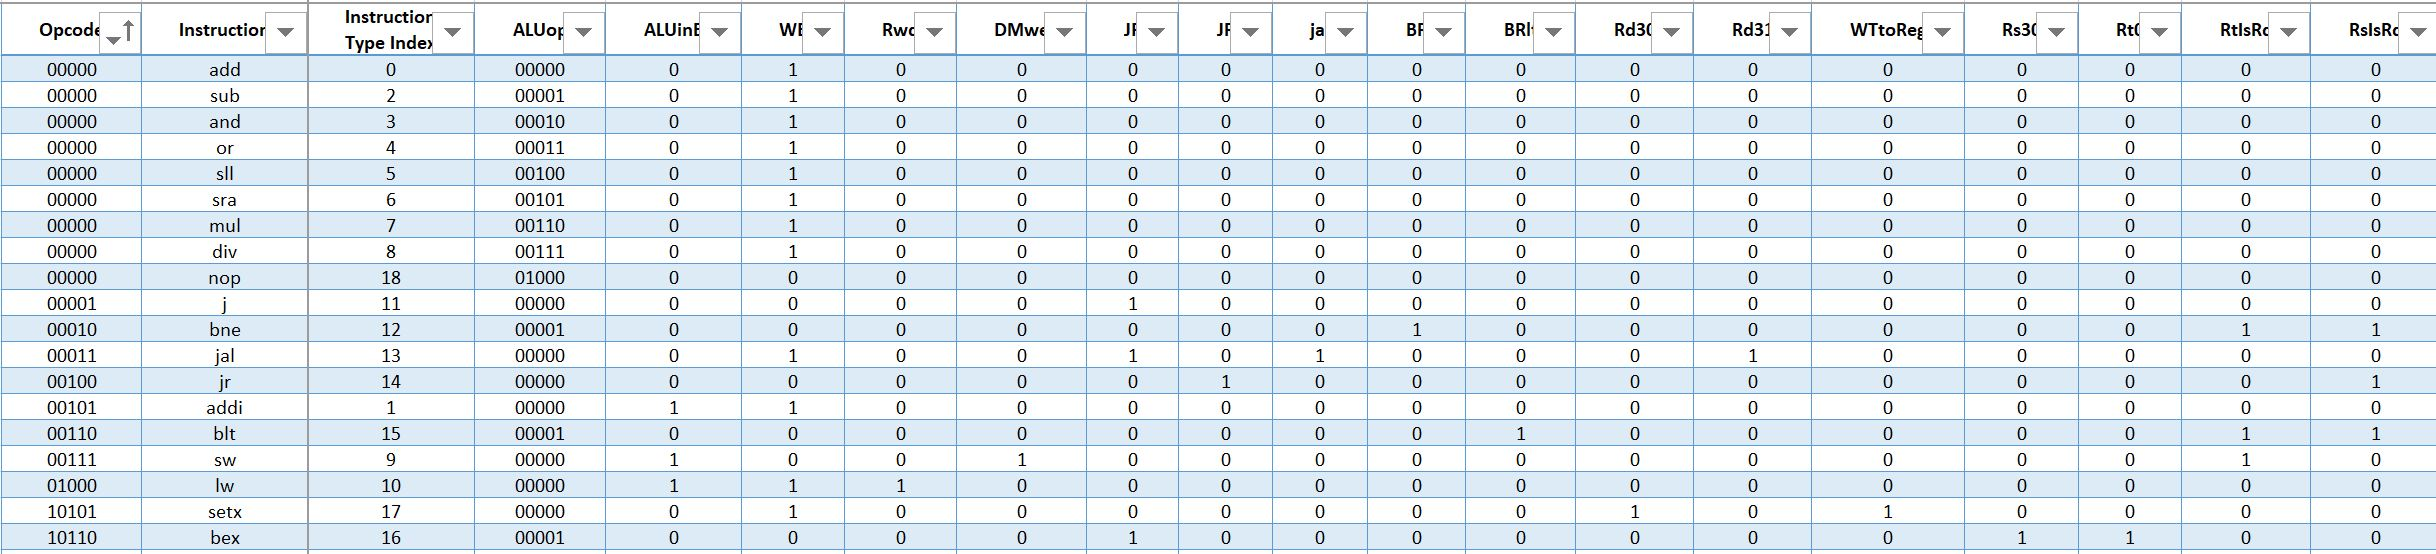
\includegraphics[width=1.2\textwidth]{InsnTable1.JPG}
\caption{Table of Control Bits for each instruction}
\label{fig:1}
\end{center}
\end{figure}

\begin{figure}[h]
\begin{center}
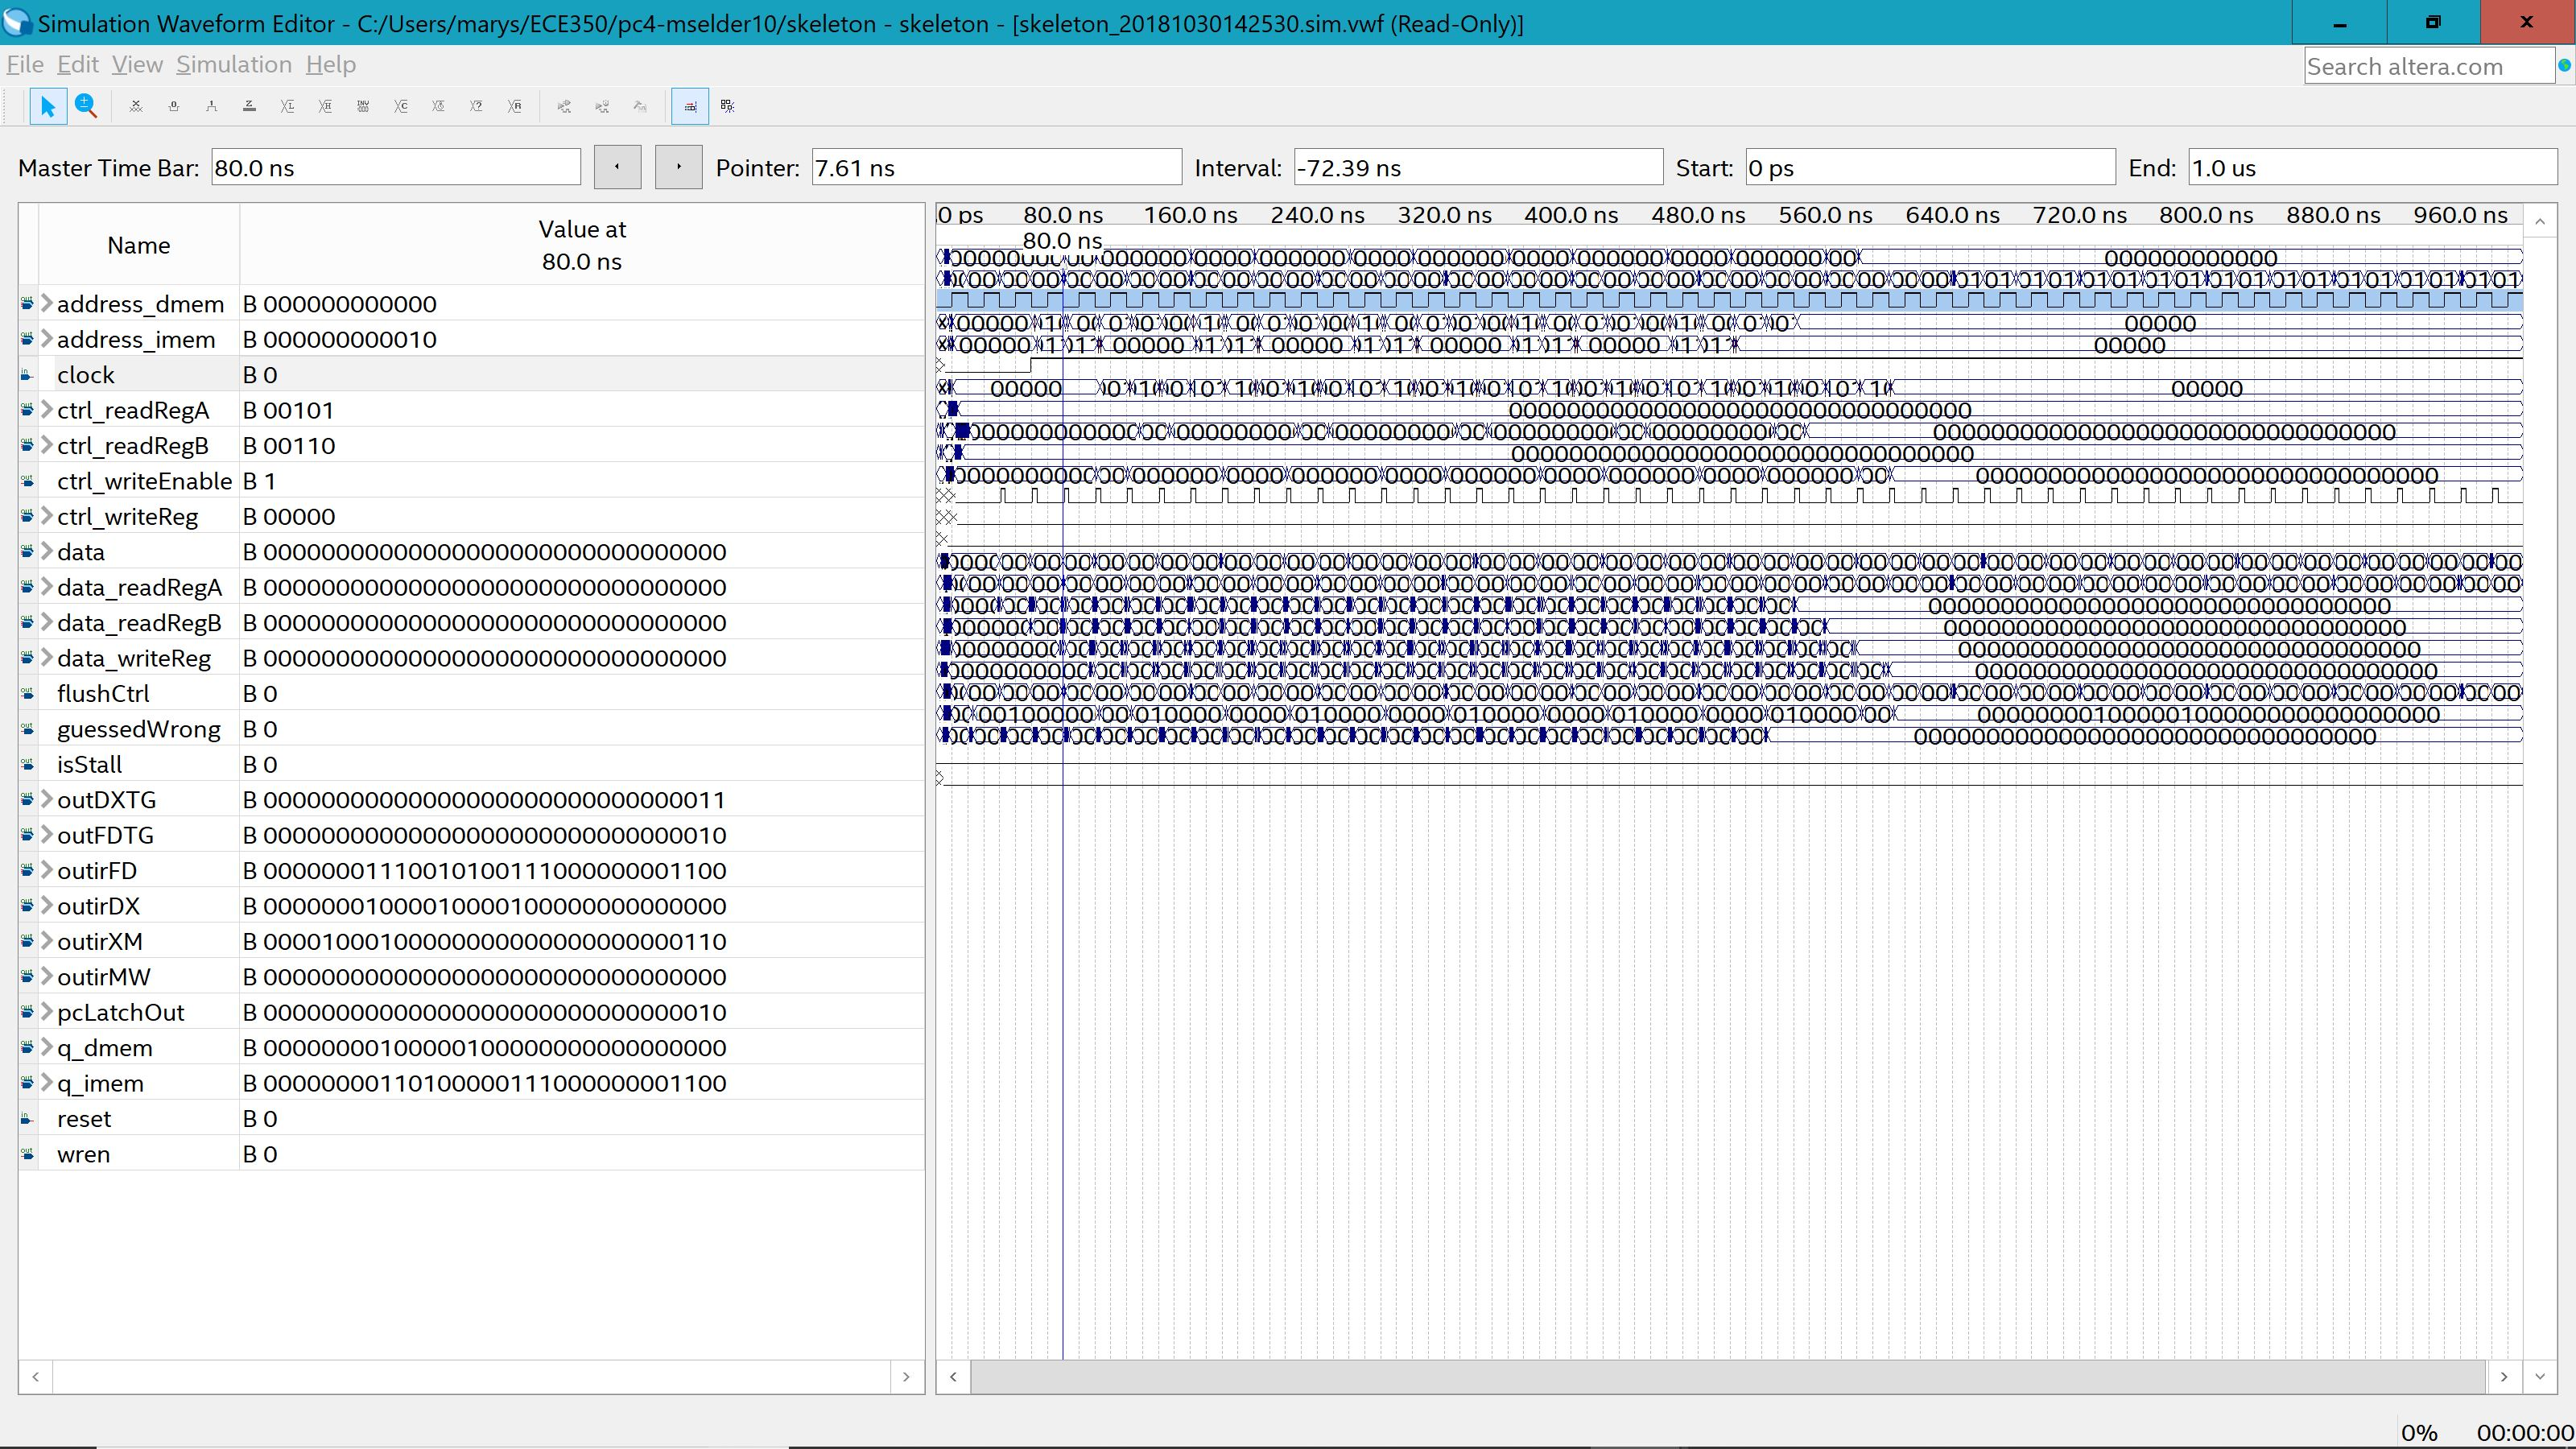
\includegraphics[width=1.2\textwidth]{0add0.JPG}
\caption{Image of Waveform for the First Instruction Through Pipeline}
\label{fig:2}
\end{center}
\end{figure}

\end{document}
